\documentclass{article} % For LaTeX2e
\usepackage{iclr2021_conference,times}

% Optional math commands from https://github.com/goodfeli/dlbook_notation.

\usepackage{amsmath,amsfonts,bm}

\newcommand{\figleft}{{\em (Left)}}
\newcommand{\figcenter}{{\em (Center)}}
\newcommand{\figright}{{\em (Right)}}
\newcommand{\figtop}{{\em (Top)}}
\newcommand{\figbottom}{{\em (Bottom)}}
\newcommand{\captiona}{{\em (a)}}
\newcommand{\captionb}{{\em (b)}}
\newcommand{\captionc}{{\em (c)}}
\newcommand{\captiond}{{\em (d)}}

\newcommand{\newterm}[1]{{\bf #1}}


\def\figref#1{figure~\ref{#1}}
\def\Figref#1{Figure~\ref{#1}}
\def\twofigref#1#2{figures \ref{#1} and \ref{#2}}
\def\quadfigref#1#2#3#4{figures \ref{#1}, \ref{#2}, \ref{#3} and \ref{#4}}
\def\secref#1{section~\ref{#1}}
\def\Secref#1{Section~\ref{#1}}
\def\twosecrefs#1#2{sections \ref{#1} and \ref{#2}}
\def\secrefs#1#2#3{sections \ref{#1}, \ref{#2} and \ref{#3}}
\def\eqref#1{equation~\ref{#1}}
\def\Eqref#1{Equation~\ref{#1}}
\def\plaineqref#1{\ref{#1}}
\def\chapref#1{chapter~\ref{#1}}
\def\Chapref#1{Chapter~\ref{#1}}
\def\rangechapref#1#2{chapters\ref{#1}--\ref{#2}}
\def\algref#1{algorithm~\ref{#1}}
\def\Algref#1{Algorithm~\ref{#1}}
\def\twoalgref#1#2{algorithms \ref{#1} and \ref{#2}}
\def\Twoalgref#1#2{Algorithms \ref{#1} and \ref{#2}}
\def\partref#1{part~\ref{#1}}
\def\Partref#1{Part~\ref{#1}}
\def\twopartref#1#2{parts \ref{#1} and \ref{#2}}

\def\ceil#1{\lceil #1 \rceil}
\def\floor#1{\lfloor #1 \rfloor}
\def\1{\bm{1}}
\newcommand{\train}{\mathcal{D}}
\newcommand{\valid}{\mathcal{D_{\mathrm{valid}}}}
\newcommand{\test}{\mathcal{D_{\mathrm{test}}}}

\def\eps{{\epsilon}}


\def\reta{{\textnormal{$\eta$}}}
\def\ra{{\textnormal{a}}}
\def\rb{{\textnormal{b}}}
\def\rc{{\textnormal{c}}}
\def\rd{{\textnormal{d}}}
\def\re{{\textnormal{e}}}
\def\rf{{\textnormal{f}}}
\def\rg{{\textnormal{g}}}
\def\rh{{\textnormal{h}}}
\def\ri{{\textnormal{i}}}
\def\rj{{\textnormal{j}}}
\def\rk{{\textnormal{k}}}
\def\rl{{\textnormal{l}}}
\def\rn{{\textnormal{n}}}
\def\ro{{\textnormal{o}}}
\def\rp{{\textnormal{p}}}
\def\rq{{\textnormal{q}}}
\def\rr{{\textnormal{r}}}
\def\rs{{\textnormal{s}}}
\def\rt{{\textnormal{t}}}
\def\ru{{\textnormal{u}}}
\def\rv{{\textnormal{v}}}
\def\rw{{\textnormal{w}}}
\def\rx{{\textnormal{x}}}
\def\ry{{\textnormal{y}}}
\def\rz{{\textnormal{z}}}

\def\rvepsilon{{\mathbf{\epsilon}}}
\def\rvtheta{{\mathbf{\theta}}}
\def\rva{{\mathbf{a}}}
\def\rvb{{\mathbf{b}}}
\def\rvc{{\mathbf{c}}}
\def\rvd{{\mathbf{d}}}
\def\rve{{\mathbf{e}}}
\def\rvf{{\mathbf{f}}}
\def\rvg{{\mathbf{g}}}
\def\rvh{{\mathbf{h}}}
\def\rvu{{\mathbf{i}}}
\def\rvj{{\mathbf{j}}}
\def\rvk{{\mathbf{k}}}
\def\rvl{{\mathbf{l}}}
\def\rvm{{\mathbf{m}}}
\def\rvn{{\mathbf{n}}}
\def\rvo{{\mathbf{o}}}
\def\rvp{{\mathbf{p}}}
\def\rvq{{\mathbf{q}}}
\def\rvr{{\mathbf{r}}}
\def\rvs{{\mathbf{s}}}
\def\rvt{{\mathbf{t}}}
\def\rvu{{\mathbf{u}}}
\def\rvv{{\mathbf{v}}}
\def\rvw{{\mathbf{w}}}
\def\rvx{{\mathbf{x}}}
\def\rvy{{\mathbf{y}}}
\def\rvz{{\mathbf{z}}}

\def\erva{{\textnormal{a}}}
\def\ervb{{\textnormal{b}}}
\def\ervc{{\textnormal{c}}}
\def\ervd{{\textnormal{d}}}
\def\erve{{\textnormal{e}}}
\def\ervf{{\textnormal{f}}}
\def\ervg{{\textnormal{g}}}
\def\ervh{{\textnormal{h}}}
\def\ervi{{\textnormal{i}}}
\def\ervj{{\textnormal{j}}}
\def\ervk{{\textnormal{k}}}
\def\ervl{{\textnormal{l}}}
\def\ervm{{\textnormal{m}}}
\def\ervn{{\textnormal{n}}}
\def\ervo{{\textnormal{o}}}
\def\ervp{{\textnormal{p}}}
\def\ervq{{\textnormal{q}}}
\def\ervr{{\textnormal{r}}}
\def\ervs{{\textnormal{s}}}
\def\ervt{{\textnormal{t}}}
\def\ervu{{\textnormal{u}}}
\def\ervv{{\textnormal{v}}}
\def\ervw{{\textnormal{w}}}
\def\ervx{{\textnormal{x}}}
\def\ervy{{\textnormal{y}}}
\def\ervz{{\textnormal{z}}}

\def\rmA{{\mathbf{A}}}
\def\rmB{{\mathbf{B}}}
\def\rmC{{\mathbf{C}}}
\def\rmD{{\mathbf{D}}}
\def\rmE{{\mathbf{E}}}
\def\rmF{{\mathbf{F}}}
\def\rmG{{\mathbf{G}}}
\def\rmH{{\mathbf{H}}}
\def\rmI{{\mathbf{I}}}
\def\rmJ{{\mathbf{J}}}
\def\rmK{{\mathbf{K}}}
\def\rmL{{\mathbf{L}}}
\def\rmM{{\mathbf{M}}}
\def\rmN{{\mathbf{N}}}
\def\rmO{{\mathbf{O}}}
\def\rmP{{\mathbf{P}}}
\def\rmQ{{\mathbf{Q}}}
\def\rmR{{\mathbf{R}}}
\def\rmS{{\mathbf{S}}}
\def\rmT{{\mathbf{T}}}
\def\rmU{{\mathbf{U}}}
\def\rmV{{\mathbf{V}}}
\def\rmW{{\mathbf{W}}}
\def\rmX{{\mathbf{X}}}
\def\rmY{{\mathbf{Y}}}
\def\rmZ{{\mathbf{Z}}}

\def\ermA{{\textnormal{A}}}
\def\ermB{{\textnormal{B}}}
\def\ermC{{\textnormal{C}}}
\def\ermD{{\textnormal{D}}}
\def\ermE{{\textnormal{E}}}
\def\ermF{{\textnormal{F}}}
\def\ermG{{\textnormal{G}}}
\def\ermH{{\textnormal{H}}}
\def\ermI{{\textnormal{I}}}
\def\ermJ{{\textnormal{J}}}
\def\ermK{{\textnormal{K}}}
\def\ermL{{\textnormal{L}}}
\def\ermM{{\textnormal{M}}}
\def\ermN{{\textnormal{N}}}
\def\ermO{{\textnormal{O}}}
\def\ermP{{\textnormal{P}}}
\def\ermQ{{\textnormal{Q}}}
\def\ermR{{\textnormal{R}}}
\def\ermS{{\textnormal{S}}}
\def\ermT{{\textnormal{T}}}
\def\ermU{{\textnormal{U}}}
\def\ermV{{\textnormal{V}}}
\def\ermW{{\textnormal{W}}}
\def\ermX{{\textnormal{X}}}
\def\ermY{{\textnormal{Y}}}
\def\ermZ{{\textnormal{Z}}}

\def\vzero{{\bm{0}}}
\def\vone{{\bm{1}}}
\def\vmu{{\bm{\mu}}}
\def\vtheta{{\bm{\theta}}}
\def\va{{\bm{a}}}
\def\vb{{\bm{b}}}
\def\vc{{\bm{c}}}
\def\vd{{\bm{d}}}
\def\ve{{\bm{e}}}
\def\vf{{\bm{f}}}
\def\vg{{\bm{g}}}
\def\vh{{\bm{h}}}
\def\vi{{\bm{i}}}
\def\vj{{\bm{j}}}
\def\vk{{\bm{k}}}
\def\vl{{\bm{l}}}
\def\vm{{\bm{m}}}
\def\vn{{\bm{n}}}
\def\vo{{\bm{o}}}
\def\vp{{\bm{p}}}
\def\vq{{\bm{q}}}
\def\vr{{\bm{r}}}
\def\vs{{\bm{s}}}
\def\vt{{\bm{t}}}
\def\vu{{\bm{u}}}
\def\vv{{\bm{v}}}
\def\vw{{\bm{w}}}
\def\vx{{\bm{x}}}
\def\vy{{\bm{y}}}
\def\vz{{\bm{z}}}

\def\evalpha{{\alpha}}
\def\evbeta{{\beta}}
\def\evepsilon{{\epsilon}}
\def\evlambda{{\lambda}}
\def\evomega{{\omega}}
\def\evmu{{\mu}}
\def\evpsi{{\psi}}
\def\evsigma{{\sigma}}
\def\evtheta{{\theta}}
\def\eva{{a}}
\def\evb{{b}}
\def\evc{{c}}
\def\evd{{d}}
\def\eve{{e}}
\def\evf{{f}}
\def\evg{{g}}
\def\evh{{h}}
\def\evi{{i}}
\def\evj{{j}}
\def\evk{{k}}
\def\evl{{l}}
\def\evm{{m}}
\def\evn{{n}}
\def\evo{{o}}
\def\evp{{p}}
\def\evq{{q}}
\def\evr{{r}}
\def\evs{{s}}
\def\evt{{t}}
\def\evu{{u}}
\def\evv{{v}}
\def\evw{{w}}
\def\evx{{x}}
\def\evy{{y}}
\def\evz{{z}}

\def\mA{{\bm{A}}}
\def\mB{{\bm{B}}}
\def\mC{{\bm{C}}}
\def\mD{{\bm{D}}}
\def\mE{{\bm{E}}}
\def\mF{{\bm{F}}}
\def\mG{{\bm{G}}}
\def\mH{{\bm{H}}}
\def\mI{{\bm{I}}}
\def\mJ{{\bm{J}}}
\def\mK{{\bm{K}}}
\def\mL{{\bm{L}}}
\def\mM{{\bm{M}}}
\def\mN{{\bm{N}}}
\def\mO{{\bm{O}}}
\def\mP{{\bm{P}}}
\def\mQ{{\bm{Q}}}
\def\mR{{\bm{R}}}
\def\mS{{\bm{S}}}
\def\mT{{\bm{T}}}
\def\mU{{\bm{U}}}
\def\mV{{\bm{V}}}
\def\mW{{\bm{W}}}
\def\mX{{\bm{X}}}
\def\mY{{\bm{Y}}}
\def\mZ{{\bm{Z}}}
\def\mBeta{{\bm{\beta}}}
\def\mPhi{{\bm{\Phi}}}
\def\mLambda{{\bm{\Lambda}}}
\def\mSigma{{\bm{\Sigma}}}

\DeclareMathAlphabet{\mathsfit}{\encodingdefault}{\sfdefault}{m}{sl}
\SetMathAlphabet{\mathsfit}{bold}{\encodingdefault}{\sfdefault}{bx}{n}
\newcommand{\tens}[1]{\bm{\mathsfit{#1}}}
\def\tA{{\tens{A}}}
\def\tB{{\tens{B}}}
\def\tC{{\tens{C}}}
\def\tD{{\tens{D}}}
\def\tE{{\tens{E}}}
\def\tF{{\tens{F}}}
\def\tG{{\tens{G}}}
\def\tH{{\tens{H}}}
\def\tI{{\tens{I}}}
\def\tJ{{\tens{J}}}
\def\tK{{\tens{K}}}
\def\tL{{\tens{L}}}
\def\tM{{\tens{M}}}
\def\tN{{\tens{N}}}
\def\tO{{\tens{O}}}
\def\tP{{\tens{P}}}
\def\tQ{{\tens{Q}}}
\def\tR{{\tens{R}}}
\def\tS{{\tens{S}}}
\def\tT{{\tens{T}}}
\def\tU{{\tens{U}}}
\def\tV{{\tens{V}}}
\def\tW{{\tens{W}}}
\def\tX{{\tens{X}}}
\def\tY{{\tens{Y}}}
\def\tZ{{\tens{Z}}}


\def\gA{{\mathcal{A}}}
\def\gB{{\mathcal{B}}}
\def\gC{{\mathcal{C}}}
\def\gD{{\mathcal{D}}}
\def\gE{{\mathcal{E}}}
\def\gF{{\mathcal{F}}}
\def\gG{{\mathcal{G}}}
\def\gH{{\mathcal{H}}}
\def\gI{{\mathcal{I}}}
\def\gJ{{\mathcal{J}}}
\def\gK{{\mathcal{K}}}
\def\gL{{\mathcal{L}}}
\def\gM{{\mathcal{M}}}
\def\gN{{\mathcal{N}}}
\def\gO{{\mathcal{O}}}
\def\gP{{\mathcal{P}}}
\def\gQ{{\mathcal{Q}}}
\def\gR{{\mathcal{R}}}
\def\gS{{\mathcal{S}}}
\def\gT{{\mathcal{T}}}
\def\gU{{\mathcal{U}}}
\def\gV{{\mathcal{V}}}
\def\gW{{\mathcal{W}}}
\def\gX{{\mathcal{X}}}
\def\gY{{\mathcal{Y}}}
\def\gZ{{\mathcal{Z}}}

\def\sA{{\mathbb{A}}}
\def\sB{{\mathbb{B}}}
\def\sC{{\mathbb{C}}}
\def\sD{{\mathbb{D}}}
\def\sF{{\mathbb{F}}}
\def\sG{{\mathbb{G}}}
\def\sH{{\mathbb{H}}}
\def\sI{{\mathbb{I}}}
\def\sJ{{\mathbb{J}}}
\def\sK{{\mathbb{K}}}
\def\sL{{\mathbb{L}}}
\def\sM{{\mathbb{M}}}
\def\sN{{\mathbb{N}}}
\def\sO{{\mathbb{O}}}
\def\sP{{\mathbb{P}}}
\def\sQ{{\mathbb{Q}}}
\def\sR{{\mathbb{R}}}
\def\sS{{\mathbb{S}}}
\def\sT{{\mathbb{T}}}
\def\sU{{\mathbb{U}}}
\def\sV{{\mathbb{V}}}
\def\sW{{\mathbb{W}}}
\def\sX{{\mathbb{X}}}
\def\sY{{\mathbb{Y}}}
\def\sZ{{\mathbb{Z}}}

\def\emLambda{{\Lambda}}
\def\emA{{A}}
\def\emB{{B}}
\def\emC{{C}}
\def\emD{{D}}
\def\emE{{E}}
\def\emF{{F}}
\def\emG{{G}}
\def\emH{{H}}
\def\emI{{I}}
\def\emJ{{J}}
\def\emK{{K}}
\def\emL{{L}}
\def\emM{{M}}
\def\emN{{N}}
\def\emO{{O}}
\def\emP{{P}}
\def\emQ{{Q}}
\def\emR{{R}}
\def\emS{{S}}
\def\emT{{T}}
\def\emU{{U}}
\def\emV{{V}}
\def\emW{{W}}
\def\emX{{X}}
\def\emY{{Y}}
\def\emZ{{Z}}
\def\emSigma{{\Sigma}}

\newcommand{\etens}[1]{\mathsfit{#1}}
\def\etLambda{{\etens{\Lambda}}}
\def\etA{{\etens{A}}}
\def\etB{{\etens{B}}}
\def\etC{{\etens{C}}}
\def\etD{{\etens{D}}}
\def\etE{{\etens{E}}}
\def\etF{{\etens{F}}}
\def\etG{{\etens{G}}}
\def\etH{{\etens{H}}}
\def\etI{{\etens{I}}}
\def\etJ{{\etens{J}}}
\def\etK{{\etens{K}}}
\def\etL{{\etens{L}}}
\def\etM{{\etens{M}}}
\def\etN{{\etens{N}}}
\def\etO{{\etens{O}}}
\def\etP{{\etens{P}}}
\def\etQ{{\etens{Q}}}
\def\etR{{\etens{R}}}
\def\etS{{\etens{S}}}
\def\etT{{\etens{T}}}
\def\etU{{\etens{U}}}
\def\etV{{\etens{V}}}
\def\etW{{\etens{W}}}
\def\etX{{\etens{X}}}
\def\etY{{\etens{Y}}}
\def\etZ{{\etens{Z}}}

\newcommand{\pdata}{p_{\rm{data}}}
\newcommand{\ptrain}{\hat{p}_{\rm{data}}}
\newcommand{\Ptrain}{\hat{P}_{\rm{data}}}
\newcommand{\pmodel}{p_{\rm{model}}}
\newcommand{\Pmodel}{P_{\rm{model}}}
\newcommand{\ptildemodel}{\tilde{p}_{\rm{model}}}
\newcommand{\pencode}{p_{\rm{encoder}}}
\newcommand{\pdecode}{p_{\rm{decoder}}}
\newcommand{\precons}{p_{\rm{reconstruct}}}

\newcommand{\laplace}{\mathrm{Laplace}} %

\newcommand{\E}{\mathbb{E}}
\newcommand{\Ls}{\mathcal{L}}
\newcommand{\R}{\mathbb{R}}
\newcommand{\emp}{\tilde{p}}
\newcommand{\lr}{\alpha}
\newcommand{\reg}{\lambda}
\newcommand{\rect}{\mathrm{rectifier}}
\newcommand{\softmax}{\mathrm{softmax}}
\newcommand{\sigmoid}{\sigma}
\newcommand{\softplus}{\zeta}
\newcommand{\KL}{D_{\mathrm{KL}}}
\newcommand{\Var}{\mathrm{Var}}
\newcommand{\standarderror}{\mathrm{SE}}
\newcommand{\Cov}{\mathrm{Cov}}
\newcommand{\normlzero}{L^0}
\newcommand{\normlone}{L^1}
\newcommand{\normltwo}{L^2}
\newcommand{\normlp}{L^p}
\newcommand{\normmax}{L^\infty}

\newcommand{\parents}{Pa} %

\DeclareMathOperator*{\argmax}{arg\,max}
\DeclareMathOperator*{\argmin}{arg\,min}

\DeclareMathOperator{\sign}{sign}
\DeclareMathOperator{\Tr}{Tr}
\let\ab\allowbreak


\usepackage{hyperref}
\usepackage{url}
\usepackage{amssymb} 
\usepackage{amsmath} 
\usepackage{amsthm} 
\usepackage{amsfonts} 
\usepackage{enumitem} 
\usepackage{tabularx} 
\usepackage{centernot}
\usepackage[parfill]{parskip}
\usepackage{quiver}

\usepackage{graphicx} 
\usepackage{scalerel}
\newtheorem{theorem}{Theorem} 

\theoremstyle{definition} 
% \newtheorem{problem}{Exercício} 
\newtheorem{definition}{Definition} 
\newtheorem{lemma}{Lemma} 
\newtheorem*{description*}{Problema} 
\newtheorem{remark}{Remark} 
\newtheorem{exercise}{Exercise} 
\newtheorem{assumption}{Assumption}
\usepackage[]{xcolor} 
 
\title{How powerful are GFlowNets?}

% Authors must not appear in the submitted version. They should be hidden
% as long as the \iclrfinalcopy macro remains commented out below.
% Non-anonymous submissions will be rejected without review.

\author{Antiquus S.~Hippocampus, Natalia Cerebro \& Amelie P. Amygdale \thanks{ Use footnote for providing further information
about author (webpage, alternative address)---\emph{not} for acknowledging
funding agencies.  Funding acknowledgements go at the end of the paper.} \\
Department of Computer Science\\
Cranberry-Lemon University\\
Pittsburgh, PA 15213, USA \\
\texttt{\{hippo,brain,jen\}@cs.cranberry-lemon.edu} \\
\And
Ji Q. Ren \& Yevgeny LeNet \\
Department of Computational Neuroscience \\
University of the Witwatersrand \\
Joburg, South Africa \\
\texttt{\{robot,net\}@wits.ac.za} \\
\AND
Coauthor \\
Affiliation \\
Address \\
\texttt{email}
}

% The \author macro works with any number of authors. There are two commands
% used to separate the names and addresses of multiple authors: \And and \AND.
%
% Using \And between authors leaves it to \LaTeX{} to determine where to break
% the lines. Using \AND forces a linebreak at that point. So, if \LaTeX{}
% puts 3 of 4 authors names on the first line, and the last on the second
% line, try using \AND instead of \And before the third author name.

\newcommand{\fix}{\marginpar{FIX}}
\newcommand{\new}{\marginpar{NEW}}

%\iclrfinalcopy % Uncomment for camera-ready version, but NOT for submission.
\begin{document}


\maketitle

\begin{abstract}
The abstract paragraph should be indented 1/2~inch (3~picas) on both left and
right-hand margins. Use 10~point type, with a vertical spacing of 11~points.
The word \textsc{Abstract} must be centered, in small caps, and in point size 12. Two
line spaces precede the abstract. The abstract must be limited to one
paragraph.
\end{abstract}



\section{Flows for trees and uniform distributions}


ping

\textcolor{blue}{
\textbf{To-do list (sensitivity analysis):}
\begin{enumerate}
    \item Sensitivity analysis for regular trees and uniform distribution 
    \item Generalization for DAGs
    \item Generalization for non-uniform distributions
\end{enumerate}
}
\textcolor{orange}{
\textbf{To-do list (policy networks):}
\begin{enumerate}
    \item Anonymous
    \begin{enumerate}
        \item Balance is impossible for some pairs of pointed DAGs and reward functions
        \item Some characterization of rewards that are particularly hard to approximate
        \item Sequences, Multisets, Anonymous and non-anonymous graphs (directed and undirected) 
\item trade-off between invariances in the networks and built into the state graphtel    \end{enumerate}
    \item Non-anonymous
\end{enumerate}
    }

\textcolor{red}{
\textbf{To-do list (evaluation and diagnostic of GFLowNets):}
\begin{enumerate}
    \item Current evaluation protocols are crap (usually focus on covering modes rather than approximation). Doing the right thing is also computationally infeasible for larges state-spaces 
    \item Convergence diagnostic based on some estimate of $\delta$, leveraging our theorems in the first part of the paper
    \item some diagonose based on, e.g, the estimates we can get from $R$ based on the trajectory-balance loss (in equilibrium, should be path independent, i.e., a constant)
\end{enumerate}
}




\subsection{Uniform distributions and uniform flows}
\begin{itemize}
    \item A uniform flow of degree $g$ and height $h$ is a Markovian flow that models a uniform distribution, meaning all the leaf nodes have the same value. The policy of such flow consists in a function that takes the incoming flow and splits it equally between each of the g outgoing nodes.
\end{itemize}

To start let us consider the example of a flow trained on a uniform distribution and policy that takes the incoming flow and split it equally to all outgoing states. The resulting uniform distribution on the terminal nodes density is  represented by $\pi^*(x)=\frac{1}{g^h}$, for each terminal object in the domain $x \in \mathcal{X}$ and $|\mathcal{X}|=g^h$.

Let us consider the case that the policy at the root of the network introduces an error in the flow of size $\delta$, meaning that one children node now will receive a flow $\frac{F}{g}+\delta$ and the other $g-1$ will continue with $\frac{F}{g}$, which is equivalent to the policy with a probability density (after normalizing) that assigns a probability $\frac{F+g\delta}{g(F+\delta)}$ to one branch and $\frac{F}{g(F+\delta)}$ to the other $g-1$ branches. The total variation distance between this new density and the original policy (uniform probability for each $g$ branches) is $\epsilon(\delta, g)=(1-\frac{1}{g})\frac{\delta}{F+\delta}$. Now we denote the resulting sampling distribution induced by this modified flow as $\pi(x)$.


\begin{figure}[h]
    \center 
% https://q.uiver.app/#q=WzAsMTMsWzMsMCwiRitcXGRlbHRhIl0sWzIsMSwiXFxmcmFje0Z9e2d9K1xcZGVsdGEiXSxbNCwxLCJcXGZyYWN7Rn17Z31cXHRleHR7IH1cXHRyaWFuZ2xlIl0sWzIsMiwiXFx0cmlhbmdsZSJdLFswLDMsIlxcZnJhY3tGfXtnXmh9K1xcZGVsdGFfMSJdLFsxLDIsIlxcdHJpYW5nbGUiXSxbNSwyLCJcXHRyaWFuZ2xlIl0sWzQsMiwiXFx0cmlhbmdsZSJdLFsxLDMsIlxcZnJhY3tGfXtnXmh9K1xcZGVsdGFfMlxcdGV4dHsgIH1cXGxkb3RzICJdLFsyLDMsIlxcZnJhY3tGfXtnXmh9K1xcZGVsdGFfe2dee2gtMX19Il0sWzQsMywiXFxmcmFje0Z9e2deaH0iXSxbNSwzLCJcXGZyYWN7Rn17Z15ofSJdLFs2LDMsIlxcZnJhY3tGfXtnXmh9Il0sWzAsMSwiXFx0ZXh0e2RlZ3JlZSBnfSJdLFswLDJdLFsyLDZdLFsyLDddLFsxLDNdLFsxLDVdLFs1LDRdLFs1LDhdLFszLDldLFs3LDEwXSxbNiwxMV0sWzYsMTJdXQ==
\[\begin{tikzcd}
	&&& {F+\delta} \\
	&& {\frac{F}{g}+\delta} && {\frac{F}{g}\text{ }\triangle} \\
	& \triangle & \triangle && \triangle & \triangle \\
	{\frac{F}{g^h}+\delta_1} & {\frac{F}{g^h}+\delta_2\text{  }\ldots } & {\frac{F}{g^h}+\delta_{g^{h-1}}} && {\frac{F}{g^h}} & {\frac{F}{g^h}} & {\frac{F}{g^h}}
	\arrow["{\text{degree g}}", from=1-4, to=2-3]
	\arrow[from=1-4, to=2-5]
	\arrow[from=2-5, to=3-6]
	\arrow[from=2-5, to=3-5]
	\arrow[from=2-3, to=3-3]
	\arrow[from=2-3, to=3-2]
	\arrow[from=3-2, to=4-1]
	\arrow[from=3-2, to=4-2]
	\arrow[from=3-3, to=4-3]
	\arrow[from=3-5, to=4-5]
	\arrow[from=3-6, to=4-6]
	\arrow[from=3-6, to=4-7]
\end{tikzcd}\]
\caption{A flow network with a extra flow of $\delta$ in one of the branches of the initial state} 
    \label{fig:tree_graph} 
\end{figure}

Let $\mu$ and $\nu$ be two probability measures, then we denote $||\mu - \nu||_{\scaleto{\textbf{TV}}{3pt}}$ as the total variation distance between them. 

\begin{assumption}\label{as: gf_tree_unif}
 Let the pair $(G_T, F)$ be a flow network such that $G_T$ is a regular tree with degree $g$ and depth $h$. Furthermore, assume that $F$ spreads uniformly in the edges of $G_T$, then the target distribution $\pi^*$ generated by $(G_T, F)$ is uniform.      
\end{assumption}

\begin{theorem}[Total variation of the sampling distribution] Let $\delta >0$ and $\sum_{i=1}^{g^{h-1}} \delta_i = \delta$, where $\delta_i \in [0, \delta]$ for all $i \in \{1,2, \dots, g^{h-1}\}$. Suppose that we have the flow network $(G_T, F+\delta)$  abiding by Assumption~\ref{as: gf_tree_unif} besides the first edge from the root to a son where it has a $\delta$ increasing generating a new target distribution $\pi$. Then under these conditions describe the total variation distance between $\pi$ and $\pi^*$ is bounded above and below by the following
\begin{align*}
& \epsilon(\delta, g) \leq ||\pi - \pi^*||_{\scaleto{\textbf{TV}}{3pt}} \leq \epsilon(\delta, g^h) \quad \text{where}
\\
& \epsilon(a,b) := \Big(1 - \frac{1}{b} \Big) \frac{a}{F+a}\,.
\end{align*}
\end{theorem}
\begin{proof}
The terminal states of the modified flow network will have two types of nodes, with flow $\frac{F}{g^h}$ and $\frac{F}{g^h}+\delta_{i}$, with $\delta_i \geq 0$ and $\sum_{i=1}^{g^{h-1}} \delta_i = \delta$. We normalize those probabilities to obtain the individual probabilities for each terminal state, which determines the density of each sample. From that, we can proceed to compute the total variation distance between $\pi$ and $\pi^*$.
\begin{align*}
    ||\pi - \pi^*||_{\scaleto{\textbf{TV}}{3pt}} &= \frac{1}{2}\sum_{x \in \mathcal{X}} | \pi(x)- \pi^*(x) | \\
                          &= \frac{1}{2}\left[(g^h-g^{h-1})\left|\frac{F}{g^h}\frac{1}{F+\delta} - \frac{1}{g^h}\right|+ \sum_{i=1}^{g^{h-1}} \left|\frac{F+g^h\delta_i}{g^h}\frac{1}{F+\delta} - \frac{1}{g^h}\right| \right] \\
                          &= \frac{1}{2}\left[\frac{g^h\delta-g^{h-1}\delta+\sum_{i=1}^{g^{h-1}}|g^h\delta_i-\delta|}{g^h(F+\delta)}\right]
\end{align*}

We can lower bound $\sum_{i=1}^{g^{h-1}}|g^h\delta_i-\delta|$, by considering that $\sum_{i=1}^{g^{h-1}}(g^h\delta_i-\delta)=g^{h}\delta-g^{h-1}\delta$, taking the absolute value of the result and each element of the sum to obtain $g^{h}\delta-g^{h-1}\delta \leq \sum_{i=1}^{g^{h-1}}|g^h\delta_i-\delta|$. Thus we obtain the lower bound 
\begin{align*}
\frac{1}{2}\left[\frac{g^h\delta-g^{h-1}\delta+g^{h}\delta-g^{h-1}\delta}{g^h(F+\delta)}\right]&\leq \frac{1}{2}\left[\frac{g^h\delta-g^{h-1}\delta+\sum_{i=1}^{g^{h-1}}|g^h\delta_i-\delta|}{g^h(F+\delta)}\right] \\
                       \left(1-\frac{1}{g}\right)\frac{\delta}{F+\delta} &\leq  ||\pi - \pi^*||_{\scaleto{\textbf{TV}}{3pt}} 
\end{align*}.

This lower bound is reached when all error terms in the terminal states have the same value $\delta_i = \frac{\delta}{g^h}$.

To upper bound $|g^h\delta_i-\delta|$ we apply the triangle inequality, obtaining $|g^h\delta_i-\delta| \leq g^h\delta_i+\delta$ and  $\sum_{i=1}^{g^{h-1}}|g^h\delta_i-\delta| \leq g^h\delta+g^{h-1}\delta$, from which we obtain the upper bound
\begin{align*}
    ||\pi - \pi^*||_{\scaleto{\textbf{TV}}{3pt}} &\leq \frac{1}{2}\left[\frac{g^h\delta-g^{h-1}\delta + g^{h}\delta+g^{h-1}\delta}{g^h(F+\delta)}\right] \\
    ||\pi - \pi^*||_{\scaleto{\textbf{TV}}{3pt}} &\leq \frac{\delta}{F+\delta}
\end{align*}.

To obtain a tighter bound we break the sum $\sum_{i=1}^{g^{h-1}}|g^h\delta_i-\delta|$ by partitioning the sum into the first $I$ terms $S_A=g^h\sum_{i=1}^{I}|\delta_i-\frac{\delta}{g^h}|$ with $\delta_i < \frac{\delta}{g^h}$ and subsequent $g^{h-1}-I$ terms $S_B=g^h\sum_{j=I+1}^{g^{h-1}}|\delta_j-\frac{\delta}{g^h}|$ with $\delta_j \geq \frac{\delta}{g^h}$. By construction, we know that $S_A+g^h\sum_{i=1}^{I}\delta_i+g^h\sum_{j=I+1}^{g^{h-1}}\delta_j-S_B=g^{h-1}\delta$, simplifying to $S_B-S_A=\delta(g^h-g^{h-1})$. We rewrite $S_A + S_B = S_B-S_A+2S_A=\delta(g^h-g^{h-1})+2S_A$, and by triangle inequality on $S_A$, we obtain the upper bound $\sum_{i=1}^{g^{h-1}}|g^h\delta_i-\delta|=S_A+S_B \leq g^h\delta-g^{h-1}\delta+2I\delta $. Setting $I=g^{h-1}-1$ (the biggest value it can have without breaking the constraints on $\delta_i$), it simplifies to $S_A+S_B \leq g^h\delta+g^{h-1}\delta-2\delta $

\begin{align*}
    ||\pi - \pi^*||_{\scaleto{\textbf{TV}}{3pt}} &\leq \frac{1}{2}\left[\frac{g^h\delta-g^{h-1}\delta+\sum_{i=1}^{g^{h-1}}|g^h\delta_i-\delta|}{g^h(F+\delta)}\right] \\
    ||\pi - \pi^*||_{\scaleto{\textbf{TV}}{3pt}} &\leq \frac{1}{2}\left[\frac{g^h\delta-g^{h-1}\delta+g^h\delta+g^{h-1}\delta-2\delta }{g^h(F+\delta)}\right] \\
    ||\pi - \pi^*||_{\scaleto{\textbf{TV}}{3pt}} &\leq \left[\frac{g^h\delta-\delta }{g^h(F+\delta)}\right] \\
    ||\pi - \pi^*||_{\scaleto{\textbf{TV}}{3pt}} &\leq  \left(1-\frac{1}{g^h}\right)\frac{\delta}{F+\delta}
\end{align*}.
\end{proof}

\textcolor{red}{\begin{theorem}[Total variation of the sampling distribution] Let $\delta >0$ and $\sum_{i=1}^{n} \delta_i = \delta$, where $\delta_i \in [0, \delta]$. Suppose that we have the flow network $(G_n, F)$ which generates a target distribution $\pi^*$ uniform in the number of final vertices. Then if we increase the flow $F$ by $\delta$ in the same graph, that is $(G_n, F + \delta)$, generating a new target distribution $\pi$, the total variation distance between $\pi$ and $\pi^*$ is bounded above and below by the following
\begin{align*}
& ||\pi -\pi^*||_{\scaleto{\textbf{TV}}{3pt}} \leq \epsilon(\delta, n) \quad \text{where}
\\
& \epsilon(a,b) := \Big(1 - \frac{1}{b} \Big) \frac{a}{F+a}\,.
\end{align*}
\end{theorem}}




\section{Inherent limitations of policy networks}



\begin{figure}
    \center 
    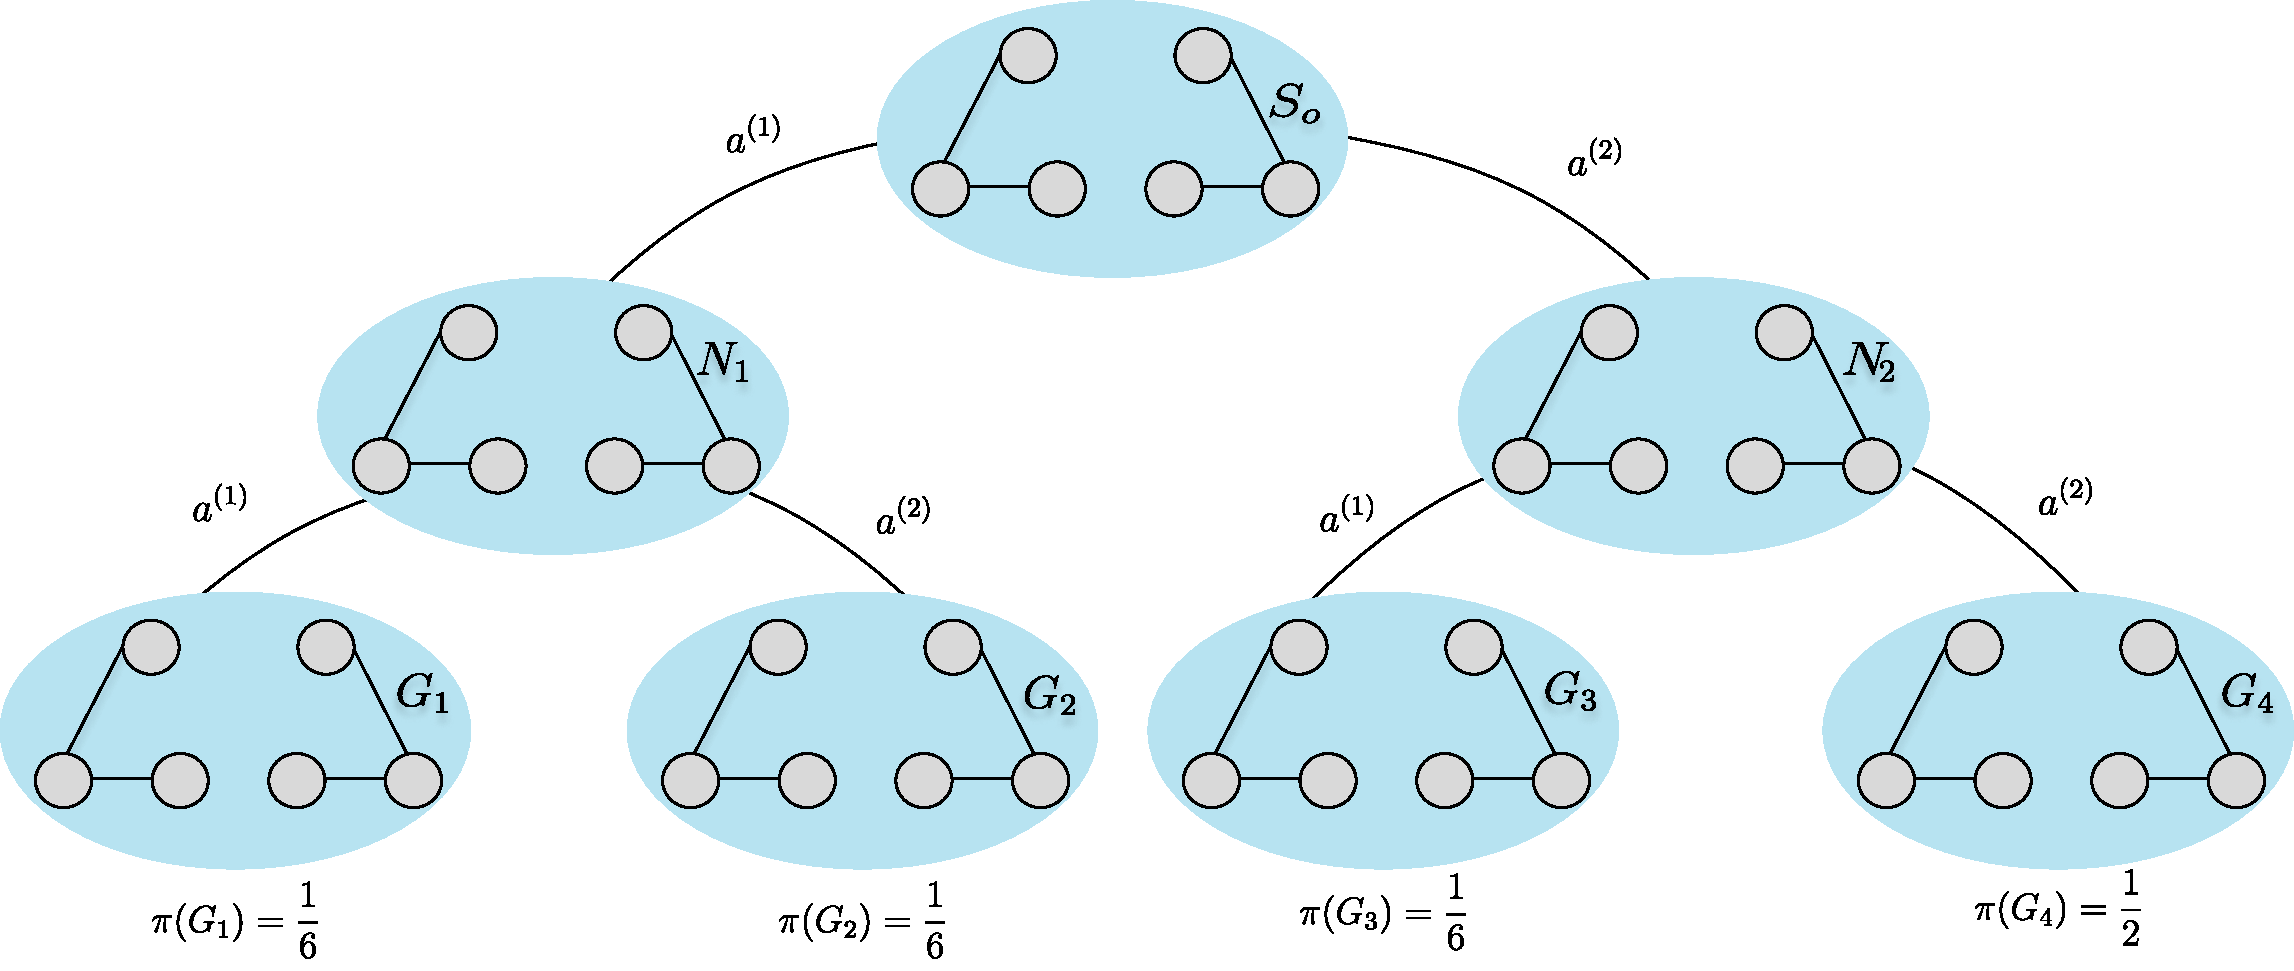
\includegraphics[scale=.3]{gflownets_wl_test.pdf} 
    \caption{A state graph whose downstream distribution is not learnable by a GFlowNet with a policy network is
    parametrized by a 1-WL GNN.} 
    \label{fig:wl_graphs} 
\end{figure}

\begin{theorem}[Distributional constraints of GFlowNets] 
    Let $\mathcal{G} = \{(\mathbf{X}, \mathbf{A}) \colon \mathbf{A} \in \{0,
    1\}^{N \times N}\}$ be the set of equally featured graphs with adjacency matrix $\mathbf{A}$
    and features $\mathbf{r} \in \mathbb{R}^{d}$ ($\mathbf{X} = \mathbf{1}\mathbf{r}^{T} \in \mathbb{R}^{N \times d}$). Let $F_{\theta} \colon \mathcal{G} \rightarrow \Delta_{2}$ be the
    \textit{policy network} that maps a graph $G \in \mathcal{G}$ to a point within the simplex of action-probabilities $\Delta_{2} =
    \{(a^{(1)}, a^{(2)}) \colon a^{(1)} + a^{(2)} = 1 \text{ and
    } a^{(1)}, a^{(2)} \ge 0\}$. See Figure~\ref{fig:wl_graphs}. Suppose that the policy network is parametrized by an 1-WL GNN with parameters $\theta$. Let $\pi$ be a distribution on the
    graphs $\{G_{i} \colon i \in \{1, 2, 3, 4\}\}$ of Figure~\ref{fig:wl_graphs} with $\pi(G_{1}) = \pi(G_{2}) = \pi(G_{3}) =
    \frac{1}{6}$ and $\pi(G_{4}) = \frac{1}{2}$. In these settings, there does not exist a
    $\theta$ such that the downstream distribution induced by the policy network equals $\pi$. 
\end{theorem}

\begin{proof}
    Let $p_{\theta}(X | S_{o})$ be the marginal transition probability learned by the GFlowNet of reaching the state $X
    \in \mathcal{G}$
    through the generative process characterized by the state graph of Figure~\ref{fig:wl_graphs} and the policy network
    $F_{\theta}$. We will show that
    $p_{\theta}(G_{i} | S_{o})$ is -- for any $\theta$ -- necessarily different of $\pi(G_{i})$ for at least two graphs
    in $\pi$'s support. 

    For this, notice that the Markovity of the stochastic transitions learned by the GFlowNet
    entails that 
    $p_{\theta}(G_{1} | S_{o}) = p_{\theta}(N_{1} | S_{o}) p_{\theta}(G_{1} | N_{1})$, 
    $p_{\theta}(G_{2} | S_{o}) = p_{\theta}(N_{1} | S_{o}) p_{\theta}(G_{2} | N_{1})$, 
    $p_{\theta}(G_{3} | S_{o}) = p_{\theta}(N_{2} | S_{o}) p_{\theta}(G_{3} | N_{2})$ and  
    $p_{\theta}(G_{4} | S_{o}) = p_{\theta}(N_{2} | S_{o}) p_{\theta}(G_{4} | N_{2})$. 
    Notably, the indistinguishability of the graphs $N_{1}$ and $N_{2}$ according to the 1-WL 
    isomorphism test implies that $F_{\theta}(N_{1}) = F_{\theta}(N_{2})$ and hence the transition  
    probabilities must satisfy $p_{\theta}(G_{1} | N_{1}) = p_{\theta}(G_{3} | N_{2})$ and $p_{\theta}(G_{2} | N_{1}) =
    p_{\theta}(G_{4} | N_{2})$. 

    Contradictorily, suppose that there is a $\theta$ such that the policy network $F_{\theta}$ is perfectly adjusted to the target distribution $\pi$.
    Hence, $p_{\theta}(G_{i} | S_{o}) = \pi(G_{i})$ for each $i \in \{1, 2, 3, 4\}$. Nonetheless, the representational equivalence of
    $N_{1}$ and $N_{2}$ and the Markovian assumption imply that 

    \begin{equation*} 
        \begin{split} 
        p_{\theta}(N_{1} | S_{o}) = \frac{\pi(G_{1})}{p_{\theta} (G_{1} | N_{1})} 
        = \frac{\pi(G_{3})}{p_{\theta} (G_{3} | N_{2})} = p_{\theta}(N_{2} | S_{o}) 
        \text{ and that } \\ 
        p_{\theta}(N_{1} | S_{o}) = \frac{\pi(G_{2})}{p_{\theta}(G_{2} | N_{1})} \neq 
        \frac{\pi(G_{4})}{p_{\theta}(G_{4} | N_{2})} = p_{\theta}(N_{2} | S_{o}).
        % p_{\theta}(N_{1} | S_{o}) = 
    \end{split} 
    \end{equation*} 

   \noindent This contradiction guarantees that $p(G_{i} | S_{o})$ is necessarily different from $\pi(G_{i})$ for at
   least a pair of graphs and asseverates that the distribution characterized by the state graph of
   Figure~\ref{fig:wl_graphs} is unlearnable by a GFlowNet parametrized by a 1-WL GNN. 
\end{proof}

\begin{remark}
    The previous theorem states the limitations of a GFlowNet parametrized by a 1-WL GNN. The alternative use of a more
    expressive yet not permutationally invariant flow parametrization would entail a factorially large increase of the
    size of the state graph, as equivalent graphs with different labelling would be treated differently by the flow
    estimator, and lead to a computationally untractable problem. The next theorem characterizes a weak relationship
    between the size of the state graph and the statistical efficiency of a maximally entropic exploratory policy within the state graph.   
\end{remark}

\subsubsection*{Author Contributions}
If you'd like to, you may include  a section for author contributions as is done
in many journals. This is optional and at the discretion of the authors.

\subsubsection*{Acknowledgments}
Use unnumbered third level headings for the acknowledgments. All
acknowledgments, including those to funding agencies, go at the end of the paper.

\cite{Bengio+chapter2007} 

\bibliography{iclr2021_conference}
\bibliographystyle{iclr2021_conference}

\appendix
\section{Appendix}
You may include other additional sections here.

\begin{theorem}[Total variation of the sampling distribution] Let $(G_n, F)$ be a flow network which should generates a target distribution $\pi$ uniform in the number of final vertices. Suppose there exists an edge in $G_n$, that is $s \to s' \in \mathbb{A}$ such that
\[  F(s)P_{F}(s' | s) - F(s')P_{B}(s|s') = \delta \,,\]
where $\delta > 0$. Then we have that $(G_n, F)$ generates a probability distribution $\mu_{\delta}$ such that
\begin{align*}
& \frac{\delta(n - d)}{2n(F + \delta)} \le ||\mu_{\delta} -\pi||_{\scaleto{\textbf{TV}}{3pt}} \leq \frac{\delta(n + dn - d)}{2n(F + \delta)} \,,
\end{align*}
where $d \in \{1,2, \dots, n-1\}$ is the number of final vertices that are descendants of $s'$. 
\end{theorem}
\begin{proof}
We define $D_{s'}$ as the set of final vertices that are descendants of $s'$. Thus we have
\begin{align}\label{eq:tv_mu_pi}
||\mu_{\delta} -\pi||_{\scaleto{\textbf{TV}}{3pt}} = \frac{1}{2} \sum_{i = 1}^n | \mu_{\delta} - n^{-1}|  = \frac{1}{2} \Big( \sum_{s'' \in D_{s'}} | \mu(s'') - n^{-1}| + \sum_{s'' \in D_{s'}^c} | \mu(s'') - n^{-1}| \Big)\,.
\end{align}

Now we will analyze it separately the two sum portions in~\eqref{eq:tv_mu_pi} starting with the second one. For $s'' \in D_{s'}^c$ we have $\mu_{\delta} (s'') = F/n(F + \delta)$ then we obtain
\begin{align*}
\sum_{s'' \in D_{s'}^c} | \mu(s'') - n^{-1}| = (n - d) \Big| \frac{F}{n(F+\delta)} - \frac{1}{n} \Big| = \frac{\delta(n - d)}{n(F + \delta)} \,.   
\end{align*}

We can rewrite $\delta$ as $\sum_{j = 1}^d \delta_j = \delta$ where $\delta_j \in [0, \delta]$ for every $j \in \{1, 2, \dots, d\}$. Now for $s_j \in D_{s'}$, where $j \in \{1,2, \dots, d\}$ we have 
\begin{equation}\label{eq:mu_dj}
\mu_{\delta} (s_j) = \frac{Fn^{-1} + \delta_j}{F + \delta} = \frac{F + n\delta_j}{n(F+\delta)} \,.   
\end{equation}

Now for the first sum portion in~\eqref{eq:tv_mu_pi} by~\eqref{eq:mu_dj} we obtain 
\begin{align*}
\sum_{s'' \in D_{s'}} \Big| \mu(s'') - \frac{1}{n} \Big| = \sum_{j = 1}^d \Big| \frac{F+n\delta_j}{n(F+\delta)} - \frac{1}{n}  \Big| = \frac{1}{n(F+\delta)} \sum_{j = 1}^d |n\delta_j - \delta|\,.    
\end{align*}

Since $|n(\delta/n) - \delta | \le |n\delta_j - \delta| \le |n\delta - \delta|$ for all $j \in \{1,2, \dots, d\}$ we have the desired result. 

\end{proof}

% \begin{theorem}[Total variation of the sampling distribution] Let $(G_n, F)$ be a flow network which should generates a target distribution $\pi$ uniform in the number of final vertices. Suppose there exists an edge in $G_n$, that is $s \to s' \in \mathbb{A}$ such that
% \begin{equation}\label{eq:loss_log_1}
% (\log(F(s)P_{F}(s' | s)) - \log(F(s')P_{B}(s|s')))^2 = \varepsilon \,,
% \end{equation}
% where $\varepsilon \ge 0$. Then we have that $(G_n, F)$ generates a probability distribution $\mu_{\varepsilon}$ such that
% \begin{align*}
% & \frac{(e^{\varepsilon^{\frac{1}{2}}} - 1)F(s' \to s)(n - d)}{2n(F + (e^{\varepsilon^{\frac{1}{2}}} - 1)F(s' \to s))} \le ||\mu_{\varepsilon} -\pi||_{\scaleto{\textbf{TV}}{3pt}} \leq \frac{(e^{\varepsilon^{\frac{1}{2}}} - 1)F(s' \to s)(n + dn - d)}{2n(F + (e^{\varepsilon^{\frac{1}{2}}} - 1)F(s' \to s))} \,,
% \end{align*}
% where $d \in \{1,2, \dots, n-1\}$ is the number of final vertices that are descendants of $s'$ and $F(s' \to s) = F(s')P_B (s|s')$. 
% \end{theorem}

% \begin{proof}
% First by~\eqref{eq:loss_log_1}  we obtain $F(s \to s') = (e^{\varepsilon^{\frac{1}{2}}} - 1)F(s' \to s)$. Thus, we have that the detailed balance condition is broken in the following way:
% \begin{equation*}
% \begin{split}
% & F(s)P_F (s'|s) = F(s')P_B (s|s') + \delta \quad \text{where}
% \\
% & \delta = (e^{\varepsilon^{\frac{1}{2}}} - 1)F(s \to s') \,.
% \end{split}
% \end{equation*}
% Hence $\delta$ is a positive constant. 


% Now we define $D_{s'}$ as the set of final vertices that are descendants of $s'$. Thus we have
% \begin{align}\label{eq:tv_mu_pi}
% ||\mu_{\varepsilon} -\pi||_{\scaleto{\textbf{TV}}{3pt}} = \frac{1}{2} \sum_{i = 1}^n | \mu_{\varepsilon} - n^{-1}|  = \frac{1}{2} \Big( \sum_{s'' \in D_{s'}} | \mu_{\varepsilon}(s'') - n^{-1}| + \sum_{s'' \in D_{s'}^c} | \mu_{\varepsilon}(s'') - n^{-1}| \Big)\,.
% \end{align}

% Now we will analyze it separately the two sum portions in~\eqref{eq:tv_mu_pi} starting with the second one. For $s'' \in D_{s'}^c$ we have $\mu_{\varepsilon} (s'') = F/n(F + \delta)$ then we obtain
% \begin{align*}
% \sum_{s'' \in D_{s'}^c} | \mu_{\varepsilon}(s'') - n^{-1}| = (n - d) \Big| \frac{F}{n(F+\delta)} - \frac{1}{n} \Big| = \frac{\delta(n - d)}{n(F + \delta)} \,.   
% \end{align*}

% We can rewrite $\delta$ as $\sum_{j = 1}^d \delta_j = \delta$ where $\delta_j \in [0, \delta]$ for every $j \in \{1, 2, \dots, d\}$. Now for $s_j \in D_{s'}$, where $j \in \{1,2, \dots, d\}$ we have 
% \begin{equation}\label{eq:mu_dj}
% \mu_{\delta} (s_j) = \frac{Fn^{-1} + \delta_j}{F + \delta} = \frac{F + n\delta_j}{n(F+\delta)} \,.   
% \end{equation}

% Now for the first sum portion in~\eqref{eq:tv_mu_pi} by~\eqref{eq:mu_dj} we obtain 
% \begin{align*}
% \sum_{s'' \in D_{s'}} \Big| \mu(s'') - \frac{1}{n} \Big| = \sum_{j = 1}^d \Big| \frac{F+n\delta_j}{n(F+\delta)} - \frac{1}{n}  \Big| = \frac{1}{n(F+\delta)} \sum_{j = 1}^d |n\delta_j - \delta|\,.    
% \end{align*}

% Since $|n(\delta/n) - \delta | \le |n\delta_j - \delta| \le |n\delta - \delta|$ for all $j \in \{1,2, \dots, d\}$ we have the desired result. 

% \end{proof}


\begin{theorem}[Total variation of the sampling distribution 1 mode]
Let $\pi$ be a probability distribution with one mode, that is, $\pi(x_M) = R/n$ and $\pi(x) = (n- R)/n(n-1)$ where $1 < R < n$.    %E: tem que adicionar esse R>1
\end{theorem}
\begin{proof}
We define $D_{s'}$ as the set of final vertices that are descendants of $s'$. Thus we have
\begin{align}\label{eq:tv_mu_pi_2}
||\mu_{\delta} -\pi||_{\scaleto{\textbf{TV}}{3pt}} = \frac{1}{2} \sum_{i = 1}^n | \mu_{\delta} - n^{-1}|  = \frac{1}{2} \Big( \sum_{s'' \in D_{s'}} | \mu(s'') - n^{-1}| + \sum_{s'' \in D_{s'}^c} | \mu(s'') - n^{-1}| \Big)\,.
\end{align}

First case $x_M \in D_{s'}$.

Now we will analyze separately the two sum portions in~\eqref{eq:tv_mu_pi_2} starting with the second one. For $s'' \in D_{s'}^c$ we have $\mu_{\delta} (s'') = F(n-R)/n(n-1)(F + \delta)$ then we obtain
\begin{align*}
\sum_{s'' \in D_{s'}^c} \Big| \mu(s'') - \frac{(n-R)}{n(n-1)}\Big| & = (n - d) \Big| \frac{F(n-R)}{n(n-1)(F+\delta)} - \frac{(n-R)}{n(n-1)} \Big| 
\\
& = \frac{\delta(n - d)(n-R)}{n(n-1)(F + \delta)} \,. 
\end{align*}

We can rewrite $\delta$ as $\sum_{j = 1}^d \delta_j = \delta$ where $\delta_j \in [0, \delta]$ for every $j \in \{1, 2, \dots, d\}$. Now for $s_j \in D_{s'}\backslash x_M$ we have 
\begin{align}\label{eq:mu_dj_2}
\begin{split}
& \mu_{\delta} (s_j) = \frac{F(n-R) + n(n-1)\delta_j}{n(n-1)(F+\delta)} \quad \text{and}
\\
& \mu_{\delta}(x_M) = \frac{FR + n\delta_M}{n(F+\delta)}\,.
\end{split}
\end{align}

Now for the first sum portion in~\eqref{eq:tv_mu_pi_2} by~\eqref{eq:mu_dj_2} we obtain 
\begin{align}\label{eq:tv_mu_pi_2a}
\begin{split}
& \sum_{s'' \in D_{s'}} | \mu(s'') - \pi(s'')| = \Big| \frac{FR + n\delta_M}{n(F+\delta)} - \frac{R}{n} \Big| +   \sum_{j = 1}^{d-1} \Big| \frac{F(n-R) + n(n-1)\delta_j}{n(n-1)(F+\delta)} - \frac{(n-R)}{n(n-1)}  \Big| 
\\
& \le \Big| \frac{n\delta_M - R\delta}{n(F+\delta)} \Big| + \sum_{j=1}^{d-1} \frac{\delta_j (n-1)n + \delta(n - R)}{n(n-1)(F+\delta)}
\\
& \le \Big| \frac{n\delta_M - R\delta}{n(F+\delta)} \Big| + \frac{(\delta - \delta_M)(n-1)n + (d-1)\delta(n - R)}{n(n-1)(F+\delta)}\,.
\end{split}
\end{align}
In~\eqref{eq:tv_mu_pi_2a} we obtain the first inequality by triangle inequality.

If we have $R \ge n/2$ we obtain
\begin{equation*}
\begin{split}
& \sum_{s'' \in D_{s'}} | \mu(s'') - \pi(s'')| = \Big| \frac{n\delta_M - R\delta}{n(F+\delta)} \Big| + \frac{(\delta - \delta_M)(n-1)n + (d-1)\delta(n - R)}{n(n-1)(F+\delta)}\,.
\\
& \le \frac{R\delta}{n(F+\delta)} + \frac{n\delta(n-1) + \delta(d-1)(n-R)}{n(n-1)(F+\delta)} \le \frac{2\delta}{F + \delta} \,.
\end{split}
\end{equation*}

Otherwise if $R < n/2$ we have
\begin{equation*}
\begin{split}
& \sum_{s'' \in D_{s'}} | \mu(s'') - \pi(s'')| = \Big| \frac{n\delta_M - R\delta}{n(F+\delta)} \Big| + \frac{(\delta - \delta_M)(n-1)n + (d-1)\delta(n - R)}{n(n-1)(F+\delta)}\,.
\\
& \le \frac{\delta (n - R)}{n(F+\delta)} + \frac{n\delta(n-1) + \delta(d-1)(n-R)}{n(n-1)(F+\delta)} 
\\
& \le \frac{\delta(n - 1)(n - R) + n \delta(n-1) + \delta(d-1)(n-R)}{n(n-1)(F+\delta)} \le \frac{\delta(n - 2R)}{n(F + \delta)} \,.
\end{split}
\end{equation*}
The last inequality we obtain by the fact that $d < n$. 

Second case $x_M \in D_{s'}^c$.

Now we will analyze separately the two sum portions in~\eqref{eq:tv_mu_pi_2} starting with the second one.
\begin{equation}\label{eq_tv_mu_pi_Dsc} 
\begin{split}
\sum_{s'' \in D_{s'}^c} | \mu(s'') - \pi(s'')| & = \Big| \frac{FR}{n(F + \delta)} - \frac{R}{n} \Big| + (n - d - 1) \Big| \frac{F(n-R)}{n(n-1)(F+\delta)} - \frac{(n-R)}{n(n-1)} \Big| 
\\
& = \frac{R\delta}{n(F+\delta)} +  \frac{\delta(n - d - 1)(n-R)}{n(n-1)(F + \delta)} \,.
\end{split}
\end{equation}

Then for the first sum portion in~\eqref{eq:tv_mu_pi_2} we obtain 
\begin{equation}\label{eq:tv_mu_pi_Ds}
\begin{split}
& \sum_{s'' \in D_{s'}} \Big| \mu(s'') - \frac{(n - R)}{n(n-1)} \Big| =  \sum_{j = 1}^{d} \Big| \frac{F(n-R) + n(n-1)\delta_j}{n(n-1)(F+\delta)} - \frac{(n-R)}{n(n-1)}  \Big| 
\\
& = \sum_{j=1}^{d} \frac{\delta_j (n-1)n + \delta(n - R)}{n(n-1)(F+\delta)} = \frac{\delta(n-1)n + d\delta(n - R)}{n(n-1)(F+\delta)} \,.
\end{split}
\end{equation}

Hence by~\eqref{eq_tv_mu_pi_Dsc} and~\eqref{eq:tv_mu_pi_Ds} we obtain the desired result. 
\end{proof}




\begin{theorem}[Total variation of the sampling distribution multiple $K$ modes]
Let $\pi$ be a probability distribution, such that $K$ states have the following distribution $\pi(x_M) = R/n$ and the others $\pi(x) = (n- KR)/n(n-K)$ where $1 < R < n$ and $K \ge 2$. Suppose that $b$ is the number of modes that are descendants of $s'$.

Then we have that $(G_n, F)$ generates a probability distribution $\mu_{\delta}$ such that
\begin{equation*}
\frac{\delta(2n^2- 2nK + 2dKR - 2dn + bn- Rbn - Rn + RK)}{2n(n-K)(F + \delta)}\le ||\mu_{\delta} -\pi||_{\scaleto{\textbf{TV}}{3pt}} \le \frac{\delta(2n^2 - K^2R - 2nK - nb + bKR)}{2n(n - K)(F + \delta)}\,. 
\end{equation*}

\end{theorem}
\begin{proof}
We define $D_{s'}$ as the set of final vertices that are descendants of $s'$ and $M$ as the set of states that are modes, hence $|M| = K$. Thus we have
\begin{align}\label{eq:tv_mu_pi_3}
\begin{split}
||\mu_{\delta} -\pi||_{\scaleto{\textbf{TV}}{3pt}} & = \frac{1}{2} \sum_{i = 1}^n | \mu_{\delta}(x_i) - \pi(x_i)|  
\\
& = \frac{1}{2} \Big( \sum_{s'' \in D_{s'}} | \mu(s'') - \pi(s'')| + \sum_{s'' \in D_{s'}^c} | \mu(s'') - \pi(s'')| \Big)\,.
\end{split}
\end{align}

Now we will analyze separately the two sum portions in~\eqref{eq:tv_mu_pi_3} starting with the second one. For $s'' \in D_{s'}^c \backslash M$, we have $\mu_{\delta} (s'') = F(n-KR)/n(n-1)(F + \delta)$. For $s'' \in D_{s'}^c \cap M$ we have $\mu_{\delta}(s'') = FR/n(F + \delta)$. Then we obtain
\begin{equation}\label{eq:tv_mu_pi_5}
\begin{split}
& \sum_{s'' \in D_{s'}^c} | \mu(s'') - \pi(s'')|  = \sum_{s'' \in D_{s'}^c \cap M} | \mu(s'') - \pi(s'')| - \sum_{s'' \in D_{s'}^c \backslash M} | \mu(s'') - \pi(s'')|
\\
& = \sum_{j = 1}^{K - b} \Big| \frac{FR}{n(F+\delta)} - \frac{R}{n} \Big| + \sum_{j = 1}^{n -K - d} \Big| \frac{F(n-KR)}{n(n-K)(F+\delta)} - \frac{(n-KR)}{n(n-K)} \Big| 
\\
& = \frac{\delta R(K-b)}{n(F+\delta)} + \frac{(n- K - d)(n - KR)\delta}{n(n - K)(F+\delta)}\,.
\end{split}
\end{equation}

We can rewrite $\delta$ as $\sum_{s'' \in D_{s'}} \delta_{s''} = \delta$ where $\delta_{s''} \in [0, \delta]$ for every $s'' \in D_{s'}$ and $|D_s'| = d$. Now for $s \in D_{s'}\backslash M$ and $x \in D_{s'} \cap M$ we have 
\begin{align}\label{eq:mu_dj_3}
\begin{split}
& \mu_{\delta} (s) = \frac{F(n-KR) + n(n-K)\delta_s}{n(n-K)(F+\delta)} \quad \text{and}
\\
& \mu_{\delta}(x) = \frac{FR + n\delta_x}{n(F+\delta)}\,.
\end{split}
\end{align}

Now for the first sum portion in~\eqref{eq:tv_mu_pi_3} by~\eqref{eq:mu_dj_3} we obtain 
\begin{align}\label{eq:tv_mu_pi_3a}
\begin{split}
& \sum_{s'' \in D_{s'}} | \mu(s'') - \pi(s'')| = \sum_{s'' \in D_{s'} \cap M}| \mu(s'') - \pi(s'')| + \sum_{s'' \in D_{s'} \backslash M} | \mu(s'') - \pi(s'')|   
\\
& = \sum_{s'' \in D_{s'} \cap M} \Big| \frac{FR + n\delta_{s''}}{n(F+\delta)} - \frac{R}{n} \Big| +  \sum_{s'' \in D_{s'} \backslash M} \Big| \frac{F(n-R) + n(n-K)\delta_{s''}}{n(n-K)(F+\delta)} - \frac{(n-KR)}{n(n-K)}  \Big| 
\\
& \le \sum_{s'' \in D_{s'} \cap M} \Big| \frac{n\delta_{s''} - R\delta}{n(F+\delta)} \Big| + \sum_{s'' \in D_{s'} \backslash M} \frac{\delta_{s''} (n-K)n + \delta(n - KR)}{n(n-K)(F+\delta)} \,.
\end{split}
\end{align}
In~\eqref{eq:tv_mu_pi_3a} we obtain the first inequality by triangle inequality.

We define $\delta_M = \sum_{s'' \in D_{s'} \cap M} \delta_{s''}$, hence $\delta_M \in [0, \delta]$ and from~\eqref{eq:tv_mu_pi_3a} we have
\begin{equation}\label{eq:tv_mu_pi_4}
\begin{split}
& \sum_{s'' \in D_{s'}} | \mu(s'') - \pi(s'')|  \le  \sum_{s'' \in D_{s'} \cap M} \Big| \frac{n\delta_{s''} - R\delta}{n(F+\delta)} \Big| +  \frac{(\delta - \delta_M) (n-K)n + \delta(d-b)(n - KR)}{n(n-K)(F+\delta)} 
\\
& \le  \sum_{s'' \in D_{s'} \cap M} \Big| \frac{n\delta_{s''} - R\delta}{n(F+\delta)} \Big|  - \frac{\delta_M}{F + \delta} + \frac{\delta n(n-K) + \delta(d-b)(n - KR)}{n(n-K)(F+\delta)} 
\\
& \le \frac{b\delta R}{n(F+\delta)} + \frac{n \delta (n - K) + \delta(d-b)(n -KR)}{n(n-K)(F + \delta)} \,.
\end{split}   
\end{equation}

Note that, in order to derive the last inequality in~\eqref{eq:tv_mu_pi_4}, it suffices to show that $\sum_{s'' \in D_{s'} \cap M} |n\delta_{s''} - R\delta| - n \delta_M \le b\delta R$ for all $\delta_M \in [0, \delta]$. Then we have
\begin{equation*}
\sum_{s'' \in D_{s'} \cap M} |n\delta_{s''} - R\delta| \le \sum_{s'' \in D_{s'} \cap M} (n\delta_{s''} + R\delta) = n\delta_M + b\delta R\,.    
\end{equation*}

Hence from~\eqref{eq:tv_mu_pi_5} and~\eqref{eq:tv_mu_pi_4} we obtain the upper bound. 

Now we will prove lower-bound. From the second equality in~\eqref{eq:tv_mu_pi_3a} we obtain
\begin{equation}\label{eq:tv_mu_pi_6}
\begin{split}
& \sum_{s'' \in D_{s'}} |\mu(s'') - \pi(s'')| \ge \sum_{s'' \in D_{s'} \cap M} \Big| \frac{n\delta_{s''} - R\delta}{n(F+\delta)} \Big| + \sum_{s'' \in D_{s'} \backslash M} \frac{\delta_{s''} (n-K)n + \delta(KR - n)}{n(n-K)(F+\delta)}
\\
& \ge \sum_{s'' \in D_{s'} \cap M} \Big| \frac{n\delta_{s''} - R\delta}{n(F+\delta)} \Big| +  \frac{(\delta - \delta_M) (n-K)n + \delta(d-b)(KR - n)}{n(n-K)(F+\delta)} 
\\
& \ge \sum_{s'' \in D_{s'} \cap M} \Big| \frac{n\delta_{s''} - R\delta}{n(F+\delta)} \Big|  - \frac{\delta_M}{F + \delta} + \frac{\delta n(n-K) + \delta(d-b)(KR - n)}{n(n-K)(F+\delta)}
\\
& \ge \frac{-R\delta}{n(F+\delta)} + \frac{\delta n(n-K) + \delta(d-b)(KR - n)}{n(n-K)(F+\delta)} \,.
\end{split}    
\end{equation}

Note that, to obtain the last inequality in~\eqref{eq:tv_mu_pi_6}, it suffices to prove that $\sum_{s'' \in D_{s'} \cap M} |n \delta_{s''} - R\delta| - n\delta_M \ge - R\delta$ for all $\delta_M \in [0, \delta]$. Then we have 
\begin{equation}\label{eq:tv_mu_pi_7}
\begin{split}
\sum_{s'' \in D_{s'} \cap M} |n \delta_{s''} - R\delta| - n\delta_M & \ge \Big| \sum_{s'' \in D_{s'} \cap M} n \delta_{s''} - R\delta \Big|  - n\delta_M
\\
& \ge |n\delta_M - R\delta| - n\delta_M \ge -R\delta \,. 
\end{split}
\end{equation}

Then we have the lower-bound by~\eqref{eq:tv_mu_pi_5} and~\eqref{eq:tv_mu_pi_7}. Hence we finished the proof. 

\end{proof}

\begin{theorem}[Total variation of the sampling distribution] Let $(G_n, F)$ be a flow network which should generates a target distribution $\pi$ with support $X$. Suppose there exists an edge in $G_n$, that is $s \to s' \in \mathbb{A}$ such that the detailed balanced condition is broken and we have
\begin{equation}\label{eq:loss_log_1}
(\log(F(s)P_{F}(s' | s)) - \log(F(s')P_{B}(s|s')))^2 = \varepsilon \,,
\end{equation}
where $\varepsilon \ge 0$. Then we have that $(G_n, F)$ generates a probability distribution $\mu_{\varepsilon}$. Let $d \in \{1,2, \dots, n-1\}$ be the number of final vertices that are descendants of $s'$ and $F(s' \to s) = F(s')P_B(s|s')$.
\begin{itemize}
    \item [i)] If $\pi$ is uniform in the number of final vertices we have
    \begin{align*}
    & \frac{(e^{\varepsilon^{\frac{1}{2}}} - 1)F(s' \to s)(n - d)}{n(F + (e^{\varepsilon^{\frac{1}{2}}} - 1)F(s' \to s))} \le ||\mu_{\varepsilon} -\pi||_{\scaleto{\textbf{TV}}{3pt}} \leq \frac{(e^{\varepsilon^{\frac{1}{2}}} - 1)F(s' \to s)(n - 1)}{n(F + (e^{\varepsilon^{\frac{1}{2}}} - 1)F(s' \to s))} \,,
    \end{align*}

    \item [ii)] If $\pi$ is a probability distribution and there exists a subset $M \subset X$ with $|M| = K$ (where $K \ge 1)$, then for each $x \in M$ we have $\pi(x_M) = R/n$ and for each $y \in X \backslash M$ we have $\pi(y) = (n- KR)/n(n-K)$ where $R < n$. Hence we obtain 

    \begin{equation*}
    \begin{split}
     &||\mu_{\delta} -\pi||_{\scaleto{\textbf{TV}}{3pt}} \ge \frac{(e^{\varepsilon^{\frac{1}{2}}} - 1)F(s' \to s)(2n^2- 2nK + 2dKR - 2dn + bn- Rbn - Rn + RK)}{2n(n-K)(F + (e^{\varepsilon^{\frac{1}{2}}} - 1)F(s' \to s))} 
     \\
     & ||\mu_{\delta} -\pi||_{\scaleto{\textbf{TV}}{3pt}} \le \frac{(e^{\varepsilon^{\frac{1}{2}}} - 1)F(s' \to s)(2n^2 - K^2R - 2nK - nb + bKR)}{2n(n - K)(F + (e^{\varepsilon^{\frac{1}{2}}} - 1)F(s' \to s))}\,.
    \end{split}     
    \end{equation*}

\end{itemize}
\end{theorem}

\begin{proof}
First, we define $D_{s'}$ as the set of final vertices that are descendants of $s'$ and by~\eqref{eq:loss_log_1}  we obtain $F(s \to s') = (e^{\varepsilon^{\frac{1}{2}}} - 1)F(s' \to s)$. Thus, we have that the detailed balance condition is broken in the following way:
\begin{equation}\label{eq:ep_var}
\begin{split}
& F(s)P_F (s'|s) = F(s')P_B (s|s') + \delta \quad \text{where}
\\
& \delta = (e^{\varepsilon^{\frac{1}{2}}} - 1)F(s \to s') \,.
\end{split}
\end{equation}
Hence $\delta$ is a positive constant. 


Now we start the proof with part $i)$. Thus we have
\begin{align}\label{eq:tv_mu_pi}
||\mu_{\varepsilon} -\pi||_{\scaleto{\textbf{TV}}{3pt}} = \frac{1}{2} \sum_{i = 1}^n | \mu_{\varepsilon} - n^{-1}|  = \frac{1}{2} \Big( \sum_{s'' \in D_{s'}} | \mu_{\varepsilon}(s'') - n^{-1}| + \sum_{s'' \in D_{s'}^c} | \mu_{\varepsilon}(s'') - n^{-1}| \Big)\,.
\end{align}

Now we will analyze it separately the two sum portions in~\eqref{eq:tv_mu_pi} starting with the second one. For $s'' \in D_{s'}^c$ we have $\mu_{\varepsilon} (s'') = F/n(F + \delta)$ then we obtain
\begin{align}\label{eq:D_s^c}
\sum_{s'' \in D_{s'}^c} | \mu_{\varepsilon}(s'') - n^{-1}| = (n - d) \Big| \frac{F}{n(F+\delta)} - \frac{1}{n} \Big| = \frac{\delta(n - d)}{n(F + \delta)} \,.   
\end{align}

We can rewrite $\delta$ as $\sum_{j = 1}^d \delta_j = \delta$ where $\delta_j \in [0, \delta]$ for every $j \in \{1, 2, \dots, d\}$. Now for $s_j \in D_{s'}$, where $j \in \{1,2, \dots, d\}$ we have 
\begin{equation}\label{eq:mu_dj}
\mu_{\varepsilon} (s_j) = \frac{Fn^{-1} + \delta_j}{F + \delta} = \frac{F + n\delta_j}{n(F+\delta)} \,.   
\end{equation}

Now for the first sum portion in~\eqref{eq:tv_mu_pi} by~\eqref{eq:mu_dj} we obtain 
\begin{equation}\label{eq:lower}
\begin{split}
\sum_{s'' \in D_{s'}} \Big| \mu_{\varepsilon}(s'') - \frac{1}{n} \Big| & = \sum_{j = 1}^d \Big| \frac{F+n\delta_j}{n(F+\delta)} - \frac{1}{n}  \Big| = \frac{1}{n(F+\delta)} \sum_{j = 1}^d |n\delta_j - \delta|
\\
& \ge \frac{1}{n(F+\delta)} \sum_{j = 1}^d n\delta_j - \delta = \frac{\delta (n -d)}{n(F + \delta)} \,.
\end{split}
\end{equation}
Important to notice that the lower bound that we compute in~\eqref{eq:lower} is the same that we have $\delta_j = \delta/d$ for all $j \in \{1, 2, \dots, d \}$.

Now for the upper bound from~\eqref{eq:mu_dj} and~\eqref{eq:lower} we obtain
\begin{equation}\label{eq:upper}
\begin{split}
& \sum_{s'' \in D_{s'}} \Big| \mu_{\varepsilon}(s'') - \frac{1}{n} \Big| =  \frac{1}{n(F+\delta)} \sum_{j = 1}^d |n\delta_j - \delta| = \frac{1}{n(F+\delta)} \sum_{j = 1}^d | n\delta_j - \delta_j + \delta_j -  \delta|
\\
& \le  \frac{1}{n(F+\delta)} \sum_{j = 1}^d |n\delta_j - \delta_j| + | \delta_j - \delta| =   \frac{1}{n(F+\delta)} \sum_{j = 1}^d (\delta_j (n-1) + \delta - \delta_j ) \le \frac{\delta(n + d - 2)}{n(F+\delta)} \,.
\end{split}    
\end{equation}
Important to notice that the upper bound that we compute in~\eqref{eq:upper} is the same that we have $\delta_j = \delta$ for one $j \in \{1, 2, \dots, d \}$ and $\delta_i = 0$ for all $i \in \{1,2, \dots, d \} \backslash \{j\}$.

Hence, from~\eqref{eq:ep_var},~\eqref{eq:tv_mu_pi},~\eqref{eq:D_s^c},~\eqref{eq:lower} and~\eqref{eq:upper} we obtain the desired result for part $i)$.

Now we will prove part $ii)$.

As in the proof of part $i)$ we will analyze separately the two sum portions in~\eqref{eq:tv_mu_pi} starting with the second one. We set $|D_{s'}^c \cap M| = b$. For $s'' \in D_{s'}^c \backslash M$, we have $\mu_{\varepsilon} (s'') = F(n-KR)/n(n-1)(F + \delta)$. For $s'' \in D_{s'}^c \cap M$ we have $\mu_{\varepsilon}(s'') = FR/n(F + \delta)$. Then we obtain
\begin{equation}\label{eq:tv_mu_pi_5}
\begin{split}
& \sum_{s'' \in D_{s'}^c} | \mu_{\varepsilon}(s'') - \pi(s'')|  = \sum_{s'' \in D_{s'}^c \cap M} | \mu_{\varepsilon}(s'') - \pi(s'')| - \sum_{s'' \in D_{s'}^c \backslash M} | \mu_{\varepsilon}(s'') - \pi(s'')|
\\
& = \sum_{j = 1}^{K - b} \Big| \frac{FR}{n(F+\delta)} - \frac{R}{n} \Big| + \sum_{j = 1}^{n -K - d} \Big| \frac{F(n-KR)}{n(n-K)(F+\delta)} - \frac{(n-KR)}{n(n-K)} \Big| 
\\
& = \frac{\delta R(K-b)}{n(F+\delta)} + \frac{(n- K - d)(n - KR)\delta}{n(n - K)(F+\delta)}\,.
\end{split}
\end{equation}

We can rewrite $\delta$ as $\sum_{s'' \in D_{s'}} \delta_{s''} = \delta$ where $\delta_{s''} \in [0, \delta]$ for every $s'' \in D_{s'}$ and $|D_s'| = d$. Now for $s \in D_{s'}\backslash M$ and $x \in D_{s'} \cap M$ we have 
\begin{align}\label{eq:mu_dj_3}
\begin{split}
& \mu_{\varepsilon} (s) = \frac{F(n-KR) + n(n-K)\delta_s}{n(n-K)(F+\delta)} \quad \text{and}
\\
& \mu_{\varepsilon}(x) = \frac{FR + n\delta_x}{n(F+\delta)}\,.
\end{split}
\end{align}

Now for the first sum portion in~\eqref{eq:tv_mu_pi} by~\eqref{eq:mu_dj_3} we obtain 
\begin{align}\label{eq:tv_mu_pi_3a}
\begin{split}
& \sum_{s'' \in D_{s'}} | \mu_{\varepsilon}(s'') - \pi(s'')| = \sum_{s'' \in D_{s'} \cap M}| \mu_{\varepsilon}(s'') - \pi(s'')| + \sum_{s'' \in D_{s'} \backslash M} | \mu_{\varepsilon}(s'') - \pi(s'')|   
\\
& = \sum_{s'' \in D_{s'} \cap M} \Big| \frac{FR + n\delta_{s''}}{n(F+\delta)} - \frac{R}{n} \Big| +  \sum_{s'' \in D_{s'} \backslash M} \Big| \frac{F(n-R) + n(n-K)\delta_{s''}}{n(n-K)(F+\delta)} - \frac{(n-KR)}{n(n-K)}  \Big| 
\\
& \le \sum_{s'' \in D_{s'} \cap M} \Big| \frac{n\delta_{s''} - R\delta}{n(F+\delta)} \Big| + \sum_{s'' \in D_{s'} \backslash M} \frac{\delta_{s''} (n-K)n + \delta(n - KR)}{n(n-K)(F+\delta)} \,.
\end{split}
\end{align}
In~\eqref{eq:tv_mu_pi_3a} we obtain the first inequality by triangle inequality.

We define $\delta_M = \sum_{s'' \in D_{s'} \cap M} \delta_{s''}$, hence $\delta_M \in [0, \delta]$ and from~\eqref{eq:tv_mu_pi_3a} we have
\begin{equation}\label{eq:tv_mu_pi_4}
\begin{split}
& \sum_{s'' \in D_{s'}} | \mu_{\varepsilon}(s'') - \pi(s'')|  \le  \sum_{s'' \in D_{s'} \cap M} \Big| \frac{n\delta_{s''} - R\delta}{n(F+\delta)} \Big| +  \frac{(\delta - \delta_M) (n-K)n + \delta(d-b)(n - KR)}{n(n-K)(F+\delta)} 
\\
& \le  \sum_{s'' \in D_{s'} \cap M} \Big| \frac{n\delta_{s''} - R\delta}{n(F+\delta)} \Big|  - \frac{\delta_M}{F + \delta} + \frac{\delta n(n-K) + \delta(d-b)(n - KR)}{n(n-K)(F+\delta)} 
\\
& \le \frac{b\delta R}{n(F+\delta)} + \frac{n \delta (n - K) + \delta(d-b)(n -KR)}{n(n-K)(F + \delta)} \,.
\end{split}   
\end{equation}

Note that, in order to derive the last inequality in~\eqref{eq:tv_mu_pi_4}, it suffices to show that $\sum_{s'' \in D_{s'} \cap M} |n\delta_{s''} - R\delta| - n \delta_M \le b\delta R$ for all $\delta_M \in [0, \delta]$. Then we have
\begin{equation*}
\sum_{s'' \in D_{s'} \cap M} |n\delta_{s''} - R\delta| \le \sum_{s'' \in D_{s'} \cap M} (n\delta_{s''} + R\delta) = n\delta_M + b\delta R\,.    
\end{equation*}

Hence from~\eqref{eq:ep_var}, ~\eqref{eq:tv_mu_pi_5} and~\eqref{eq:tv_mu_pi_4} we obtain the upper bound. 

Now we will prove lower-bound. From the second equality in~\eqref{eq:tv_mu_pi_3a} we obtain
\begin{equation}\label{eq:tv_mu_pi_6}
\begin{split}
& \sum_{s'' \in D_{s'}} |\mu_{\varepsilon}(s'') - \pi(s'')| \ge \sum_{s'' \in D_{s'} \cap M} \Big| \frac{n\delta_{s''} - R\delta}{n(F+\delta)} \Big| + \sum_{s'' \in D_{s'} \backslash M} \frac{\delta_{s''} (n-K)n + \delta(KR - n)}{n(n-K)(F+\delta)}
\\
& \ge \sum_{s'' \in D_{s'} \cap M} \Big| \frac{n\delta_{s''} - R\delta}{n(F+\delta)} \Big| +  \frac{(\delta - \delta_M) (n-K)n + \delta(d-b)(KR - n)}{n(n-K)(F+\delta)} 
\\
& \ge \sum_{s'' \in D_{s'} \cap M} \Big| \frac{n\delta_{s''} - R\delta}{n(F+\delta)} \Big|  - \frac{\delta_M}{F + \delta} + \frac{\delta n(n-K) + \delta(d-b)(KR - n)}{n(n-K)(F+\delta)}
\\
& \ge \frac{-R\delta}{n(F+\delta)} + \frac{\delta n(n-K) + \delta(d-b)(KR - n)}{n(n-K)(F+\delta)} \,.
\end{split}    
\end{equation}

Note that, to obtain the last inequality in~\eqref{eq:tv_mu_pi_6}, it suffices to prove that $\sum_{s'' \in D_{s'} \cap M} |n \delta_{s''} - R\delta| - n\delta_M \ge - R\delta$ for all $\delta_M \in [0, \delta]$. Then we have 
\begin{equation*}
\begin{split}
\sum_{s'' \in D_{s'} \cap M} |n \delta_{s''} - R\delta| - n\delta_M & \ge \Big| \sum_{s'' \in D_{s'} \cap M} n \delta_{s''} - R\delta \Big|  - n\delta_M
\\
& \ge |n\delta_M - R\delta| - n\delta_M \ge -R\delta \,. 
\end{split}
\end{equation*}

Then we have the lower-bound by~\eqref{eq:ep_var}, ~\eqref{eq:tv_mu_pi_5} and~\eqref{eq:tv_mu_pi_6}. Hence we finished the proof. 


\end{proof}









\end{document}
